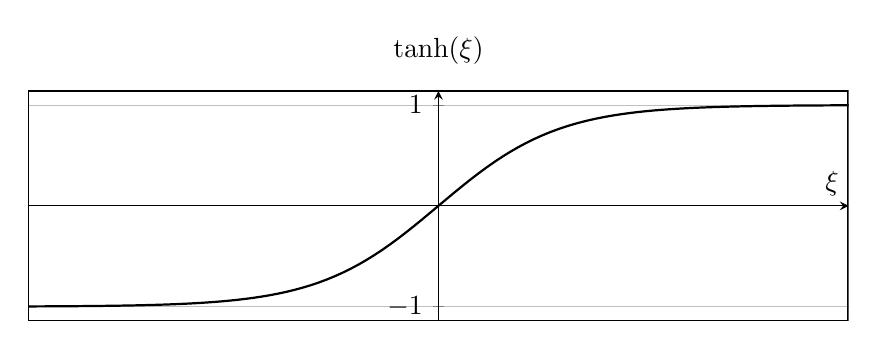
\begin{tikzpicture}
  \begin{axis}[
      samples=121,
      xmin=-3,
      xmax=3,
      ymin=-1,
      ymax=1,
      width=12cm,
      height=4.5cm,
      disabledatascaling,
      grid=both,
      %font=\footnotesize,
      %grid style={line width=.1pt, draw=red},
      %major grid style={line width=.2pt,draw=gray!50},
      %minor tick num=1,
      axis lines=middle,enlargelimits=0.07,
      %execute at begin axis={
      execute at end axis={        \draw[thick] (rel axis cs:0,0) -- (rel axis cs:1,0) -- (rel axis cs:1,1) -- (rel axis cs:0,1) --cycle;},
      %xticklabels={},
      %yticklabels={},
      xtick={-10,0,10},
      ytick={-10,-9,...,10},
      %ylabel={$\tanh(\xi)$},
      xlabel={$\xi$},
      title={$\tanh(\xi)$},
      %legend pos=south east,
    ]

    \addplot [thick, domain=-4:4] ({x}, {tanh(x)});
    %\node[anchor=south,rotate=90] at (0,-.2) {$\xi$};
  \end{axis}
\end{tikzpicture}
